\chapter{Analytical Forces Induced by Dislocations on Linear Rectangular Surface Elements}
\label{c:lin_rect}
	%
	\section{Forces Exerted by a Dislocation Line Segment on Linear Rectangular Surface Elements}
	\label{s:f_lin_rect}
		%
		\begin{figure}
			\centering
			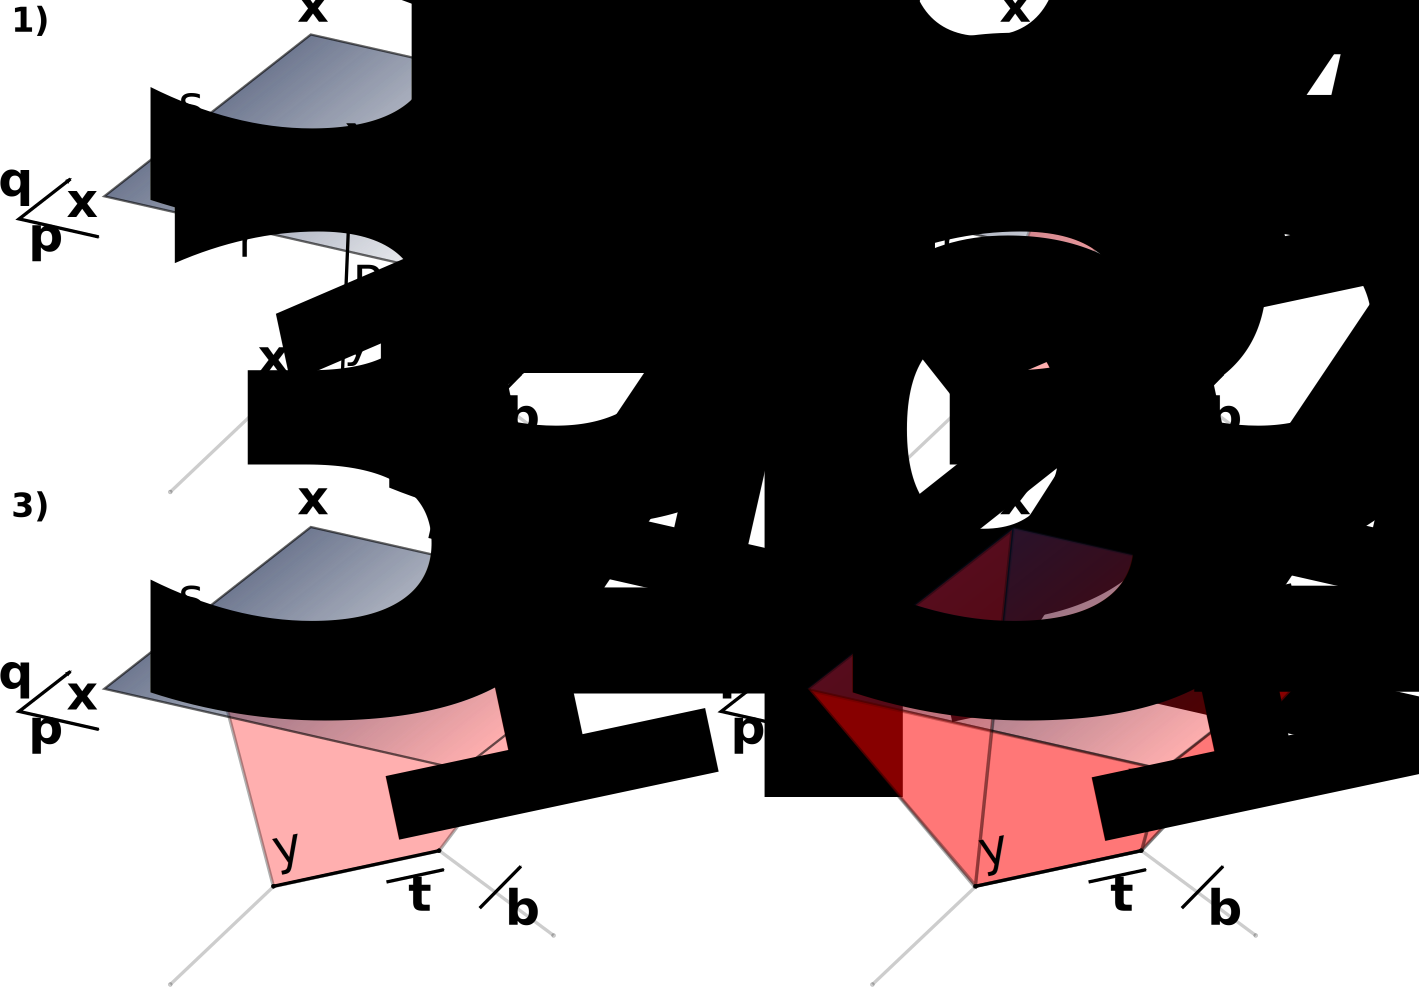
\includegraphics[width=\linewidth]{force_calc_linear_rectangle.pdf}
			\caption[Diagram of the analytical force calculation on linear rectangular surface elements.]{Diagram of the line integral method used to find analytical expressions for the forces exerted by \kwdp{dl} on linear rectangular \kwdp{se} \cite{analytical_integration_of_the_forces_induced_by_dislocations_on_a_surface_element}.
				\textit{1}) For any given point $ \vec{x} $ on the \kwd{se} and any given point $ \vec{x'}$ on the \kwd{dls}, define distance $ R_{a} $.
				\textit{2}) Integrate from $ x_{1} \to x_{2} $ along line direction $ \vec{t} $.
				\textit{3}) Integrate from $ r_{1} \to r_{2} $ along vector $ \vec{p} $.
				\textit{4}) Integrate from $ s_{1} \to s_{2} $ along vector $ \vec{q} $.}
			\label{f:flrs}
		\end{figure}
		\subsection{Resolving Singularities when Dislocation Line Segments are Parallel to Surface Elements}
		\label{ss:par_dln_se}
			%
			\begin{figure}
				\centering
				\includegraphics[width=\linewidth]{ftot_rotation_lin_rect.pdf}
				\caption[Avoiding singularities by rotating dislocation line segments.]{Effects of rotating a single \kwd{dls} on the forces exerted by it on a linear rectangular \kwd{se}. The specific values of this function are not known \emph{a priori}, all that is known is that it must be periodic ($ T = 2\pi$) and have finite maximum and minimum values. The singularity is avoided by perturbing the angle $ \theta = 0 \to \theta = \pm \epsilon\,\, \epsilon \gtrsim 0 $.}
				\label{f:rflrs}
			\end{figure}
		%
\savearabiccounter